\documentclass{_mypackages/monograph}

\title{Formation and Evolution of Galaxies \\ Problem Set 01 \\ Properties} % \MyTitle
\author{Bruno Murino - 8944901} % \MyAuthor
\date{\today} % \MyDate

\addbibresource{qinfo.bib}
\graphicspath{ {figures/} }

\begin{document}
\frontmatter

% \monographtp
% \dominitoc
% \doparttoc
% \pagestyle{onlypagenum}
% \tableofcontents

\mainmatter

\chapter{Distance between the Virgo and the Coma clusters}

Faber\footnote{Sandra Moore Faber (December 28, 1944 - ).} and Jackson\footnote{Robert Earl Jackson (1949 - ).}, in 1976\footfullcite{1976ApJ...204..668F}, noticed that the luminosity of an elliptical galaxy is correlated with its central velocity dispersion:
\begin{equation}
    L \propto \sigma_0^\beta \qq{with} beta \sim 4
\end{equation}

Thus if the apparent luminosity of two galaxies with the same central velocity dispersion is given, we can find the ratio between their distance.

\begin{figure}
    \centering
    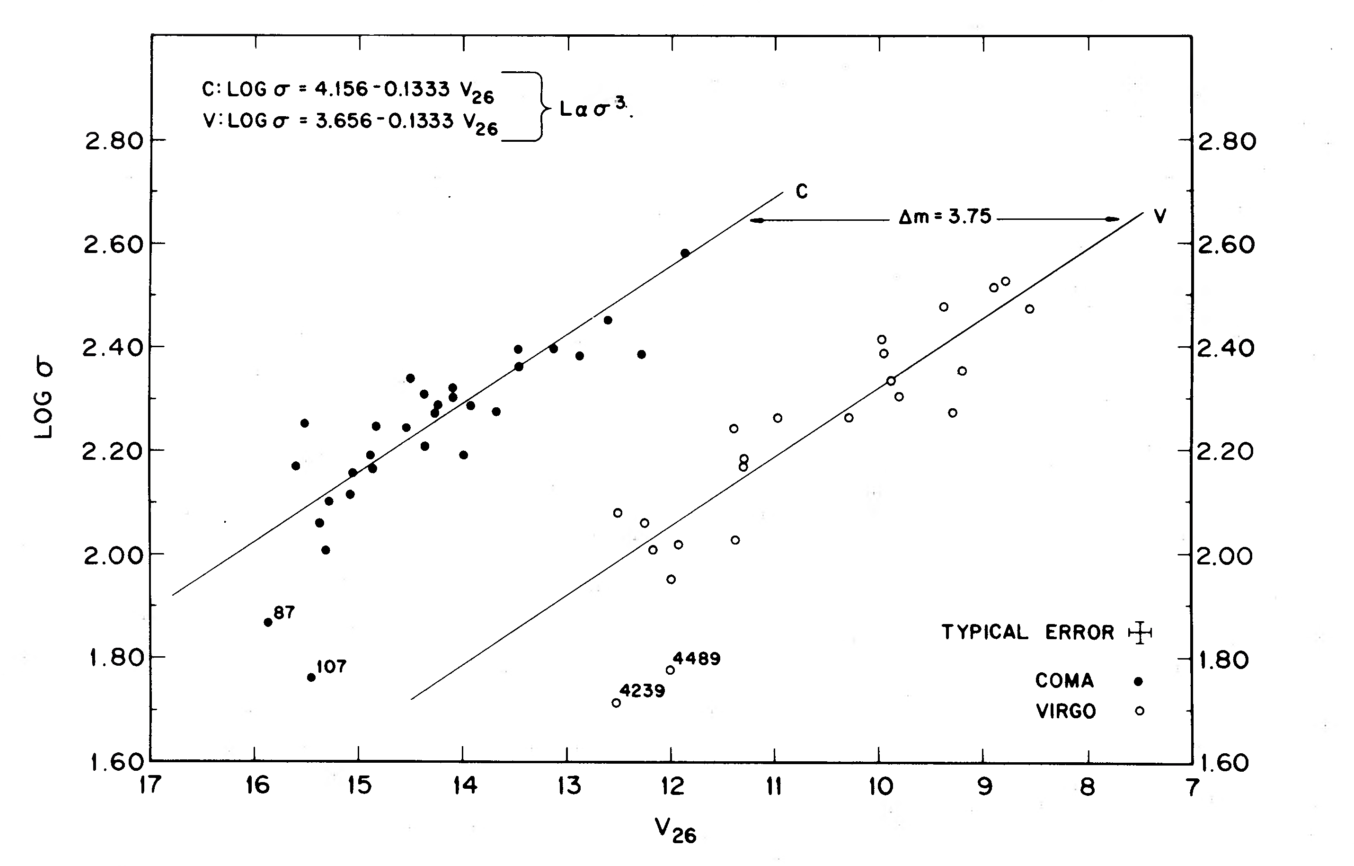
\includegraphics[width=\textwidth]{Cosmology/figures/faber-jackson.png}
    \caption{The log of the velocity dispersion vs. V26 for the Coma and Virgo ellipticals. The lines represent median fits, as described in the text, and are separated by 3.75 mag, indicating a distance ratio D(Coma)/D(Virgo) = 5.62. This implies a peculiar Virgocentric velocity of 311 km s-1. Some of the more deviant points are identified. (from \cite{Dressler1984}).}
    \label{fig:faber-jackson}
\end{figure}

From figure \ref{fig:faber-jackson} we can compare the apparent magnitude of the Virgo and Coma clusters when their central velocity dispersion is the same and find it to be around \(\num{3.75}\).

Now, taking the distance modulus equation for both clusters we find
\begin{gather}
    m_V - M_V = 5 \log_{10} \left( \frac{d_V}{\SI{10}{\parsec}}\right) \\
    m_C - M_C = 5 \log_{10} \left( \frac{d_C}{\SI{10}{\parsec}}\right)
\end{gather}
Since we will read the apparent magnitudes from \ref{fig:faber-jackson} when their central velocity distribution is the same, their absolute magnitude will be the same, thus subtracting one equation from the other we find
\begin{equation}
    m_V - m_C - (M_V - M_C) = m_V - m_C = 5 \log_{10} \left( \frac{d_V}{d_C}\right)
\end{equation}
but since \(m_V - m_C = -3.75\), we find that \(\nicefrac{d_C}{d_V} = 5.62\), which means that the Virgo cluster is closer to us than the Coma cluster.

\chapter{Baryonic density}

\begin{figure}[H]
    \centering
    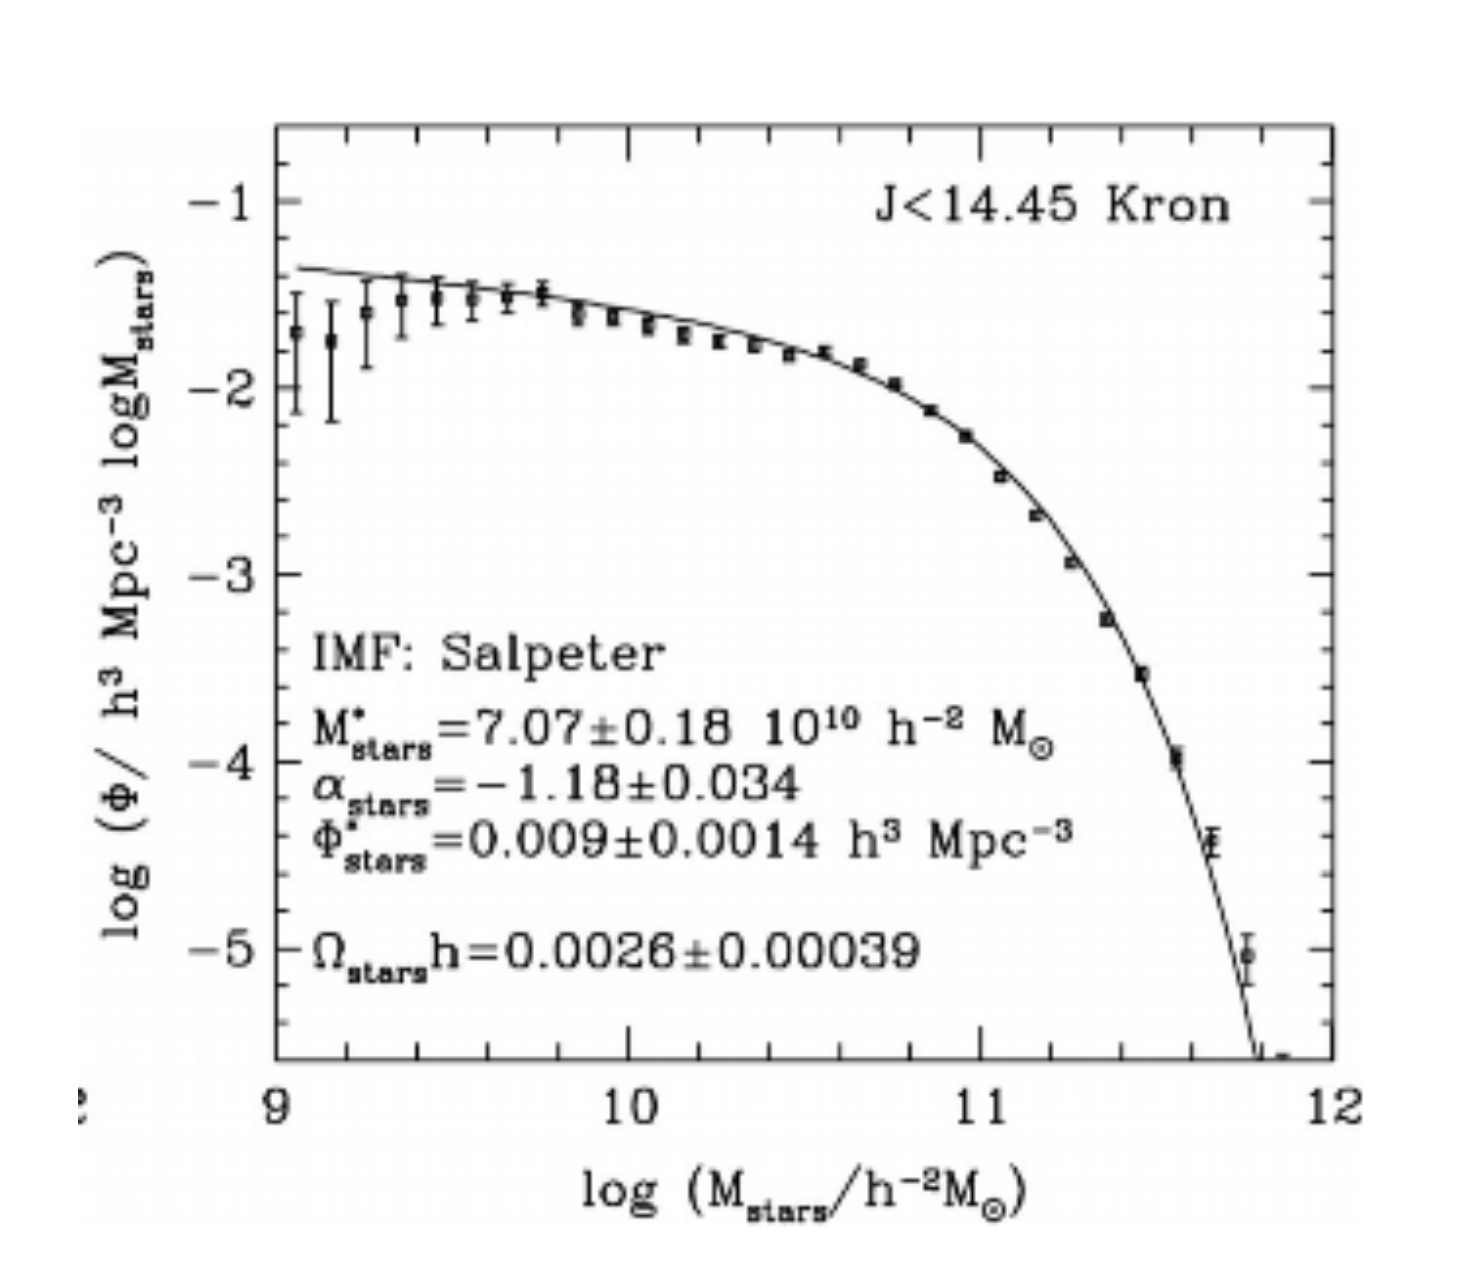
\includegraphics[width=0.8\textwidth]{Cosmology/figures/stellarmassdist.png}
    \caption{The distribution of stellar mass in galaxies in the local universe is well fitted by a Schechter function with the parameters shown in the figure.}
    \label{fig:stellarmassdist}
\end{figure}

The Schechter mass function is
\begin{equation}
    \phi(M)\dd{M} = \phi^* \bigg(\frac{M}{M_*} \bigg)^\alpha \lexp{-\frac{M}{M_*}}\frac{\dd{M}}{M_*}.
\end{equation}
and it represents the number of stars with mass between \(M\) and \(M+\dd{M}\) per unit volume. If we integrate it over all possible masses, i.e. integrate from \(0\) to \(\infty\), we will find the number of stars per unit volume (density of galaxies). If we integrate it weighted by \(M\), we will find the \emph{mass of stars per unit volume}, i.e. the stellar mass density \(\rho_s\). Lets do this.

The integral of the Schechter function weighted by \(M\) is
\begin{equation}
\begin{split}
    \rho_s &= \int_0^\infty M \phi^* \bigg(\frac{M}{M_*} \bigg)^\alpha \lexp{-\frac{M}{M_*}}\frac{\dd{M}}{M_*} \\
    &= M_* \phi^*  \int_0^\infty \bigg(\frac{M}{M_*} \bigg)^{\alpha+1} \lexp{-\frac{M}{M_*}} \dd{\left(\frac{M}{M_*}\right)},
\end{split}
\end{equation}
now writing \(\alpha+1=\beta-1\) and \(M/M_* = \gamma\), we find that
\begin{equation}
    \rho_s = M_* \phi^* \int_0^\infty \gamma^{\beta-1} \exp{-\gamma} \dd{\gamma} = M_* \phi^*\Gamma(\beta) = M_* \phi^*\Gamma(\alpha+2)
\end{equation}

Reading off the parameters \(M_*\), \(\phi^*\) and \(\alpha\) from figure \ref{fig:stellarmassdist}, we can compute \(\rho_s\):
\begin{equation}
    \rho_s = \SI{7.07}{10^{10} h^{-2} \solarmass} * \SI{0.009}{h^3 \per\mega\parsec\cubic}*\Gamma(0.82) = \SI{72}{10^7 h \solarmass \per\mega\parsec\cubic}.
\end{equation}
Dividing \(\rho_s\) by \(\rho_{\text{crit},0}\)
\begin{equation}
    \rho_{\text{crit},0} = \SI{2.775}{10^{11}h^2 \solarmass \per \mega\parsec\cubic}
\end{equation}
we find a stellar mass density of
\begin{equation}
    \Omega_{\text{stellar}} = 0.0026.
\end{equation}
Compared to the baryonic density \(\Omega_{\text{b}} = 0.022\), we conclude that only around \(12\%\) of the universe baryonic mass is in the form of stars.

\chapter{Star formation rate}

Galaxies are mostly composed of stars and between them there are two things: \emph{gas} and \emph{dust}. Together, the gas and dust are called the \emph{interstellar medium} usually abbreviated as \emph{ISM}.

The ISM gas is mostly composed of atomic hydrogen (\(H\) atom) and molecular hydrogen (\(H_2\) atom) and corresponds to about 99\% of the ISM, but all this gas isn't uniformly distributed across the galaxy, it is concentrated into clouds with a wide range of masses and sizes. Clouds composed of atomic hydrogen are denoted HI, while HII clouds are ISM gas composed of ionised atomic hydrogen, i.e. free protons.

The ISM dust is composed of small solid particles which originated in dense, relatively cool environments such as the atmospheres of red giant stars, and are released into the interstellar medium by radiation pressure, stellar winds or in material thrown off in stellar explosions.

Typical interstellar dust grains are about the same size as the wavelength of blue light meaning that they absorb and scatter UV and blue light much more efficiently than red light. The result is that light passing through a dust cloud has its blue component effectively removed, making it appear redder than it would have been otherwise. This is known as interstellar reddening. It also means that light scattered off dust grains will be blue in colour.

However, the presence of ISM dust is vital to star formation.

Since stars form from the gravitational collapse of the molecular clouds, we need molecular clouds with high density of particles, which is easier to occur on cold clouds. One of the processes that prevents the formation of big molecular clouds is the absorption of ionising radiation by hydrogen atoms, thus minimising this process helps star formation. Due to the particularly small size of dust grains, the dust part of the ISM can absorb much of this ionising radiation. Since most of this ionising radiation is composed of Lyman continuum photons\footnote{Lyman continuum photons are the photons emitted from stars at photon energies above the Lyman limit. Hydrogen is ionised by absorbing Lyman continuum photons.}, this process is called the \emph{extinction of Lyman continuum photons}. On the other hand, upon ionisation the emission of H\(\alpha\) is more present. Thus the extinction of Lyman continuum photons decreases the H\(\alpha\) luminosity. Another consequence is that, since dust absorbs radiation, it gets hotter, and then emits IR photons. Also, dust makes the formation of \(H_2\) by two hydrogen atoms more likely to happen, acting as a catalyst of the reaction.

All the above processes are taken into account by the IHK \cite{Inoue2000} analytic formula for the star formation rate, which is parameterized by \(f\), the  fraction of Lyman continuum luminosity absorbed by hydrogen atoms, \(\epsilon\), the nonionising photons from young stars (young stars emit UV light) absorbed by dust and \(\eta\), the fraction of IR luminosity originating from dust heating by old stars. By means of photometry, these parameters can be estimated.

\chapter{Stellar mass function}

To compute the stellar mass function of a galaxy we first measure its luminosity function. We then use the mass-to-light ratio to compute the mass function. We treat each galaxy type on its own since its behaviours are unique.

The mass-to-light ratio usually depends on the luminosity function of the galaxy, and age, type and metallicity of the galaxy. By means of a IMF (initial mass function), we estimate the population of stars of a galaxy and then we relate it with the luminosity to obtain the stellar mass function.

\backmatter
\printbib
\end{document}
